\documentclass[tikz,border=6pt]{standalone}
% Shared visual language for the original benchmark atlas.
\usepackage[T1]{fontenc}
\usepackage{lmodern}
\usepackage{amsmath,amssymb}
\usetikzlibrary{arrows.meta,calc,positioning,shapes.geometric,patterns,decorations.pathmorphing,backgrounds,fit}
\definecolor{ink}{HTML}{173948}
\definecolor{flow}{HTML}{167D9A}
\definecolor{control}{HTML}{A65217}
\definecolor{measure}{HTML}{70518A}
\definecolor{pale}{HTML}{EAF2F5}
\definecolor{muted}{HTML}{526571}
\definecolor{utility}{HTML}{2E8665}
\tikzset{
  every node/.style={font=\sffamily\small,text=ink},
  equipment/.style={draw=ink,line width=1pt,fill=pale,rounded corners=2pt},
  process/.style={draw=flow,line width=1.2pt,-{Latex[length=2.5mm]}},
  signal/.style={draw=control,line width=.8pt,dashed,-{Latex[length=2mm]}},
  util/.style={draw=utility,line width=1pt,-{Latex[length=2.2mm]}},
  dimension/.style={draw=muted,line width=.6pt,{Latex[length=1.7mm]}-{Latex[length=1.7mm]}},
  labelbox/.style={fill=white,inner sep=2pt,font=\sffamily\footnotesize,align=center},
  annotation/.style={font=\sffamily\footnotesize,text=muted,align=left},
  panel/.style={draw=ink!20,fill=ink!2,rounded corners=3pt,inner sep=6pt},
  instrument/.style={circle,draw=measure,fill=white,line width=.8pt,minimum size=8mm,inner sep=1pt,font=\sffamily\scriptsize,align=center},
  port/.style={circle,fill=flow,inner sep=1.6pt},
  box/.style={equipment,minimum width=3cm,minimum height=1cm,align=center},
}
\newcommand{\atlasheader}[3]{%
  \node[anchor=north west,font=\sffamily\bfseries\LARGE] at (0,0) {#1};%
  \node[anchor=north west,font=\sffamily\small,text=muted] at (0,-.75) {Paper section #2: \textit{#3}};%
  \draw[ink!25,line width=.7pt] (0,-1.25)--(26,-1.25);%
}
\newcommand{\atlasfooter}[1]{%
  \draw[ink!25,line width=.5pt] (0,-15.8)--(26,-15.8);%
  \node[anchor=north west,annotation,text width=25.8cm] at (0,-16) {#1\\Original explanatory drawing. Source: Kroll \& Schulte (2014), DOI: 10.1016/j.asoc.2014.08.034. Model variants are identified in the accompanying case sheet.};%
}

\begin{document}
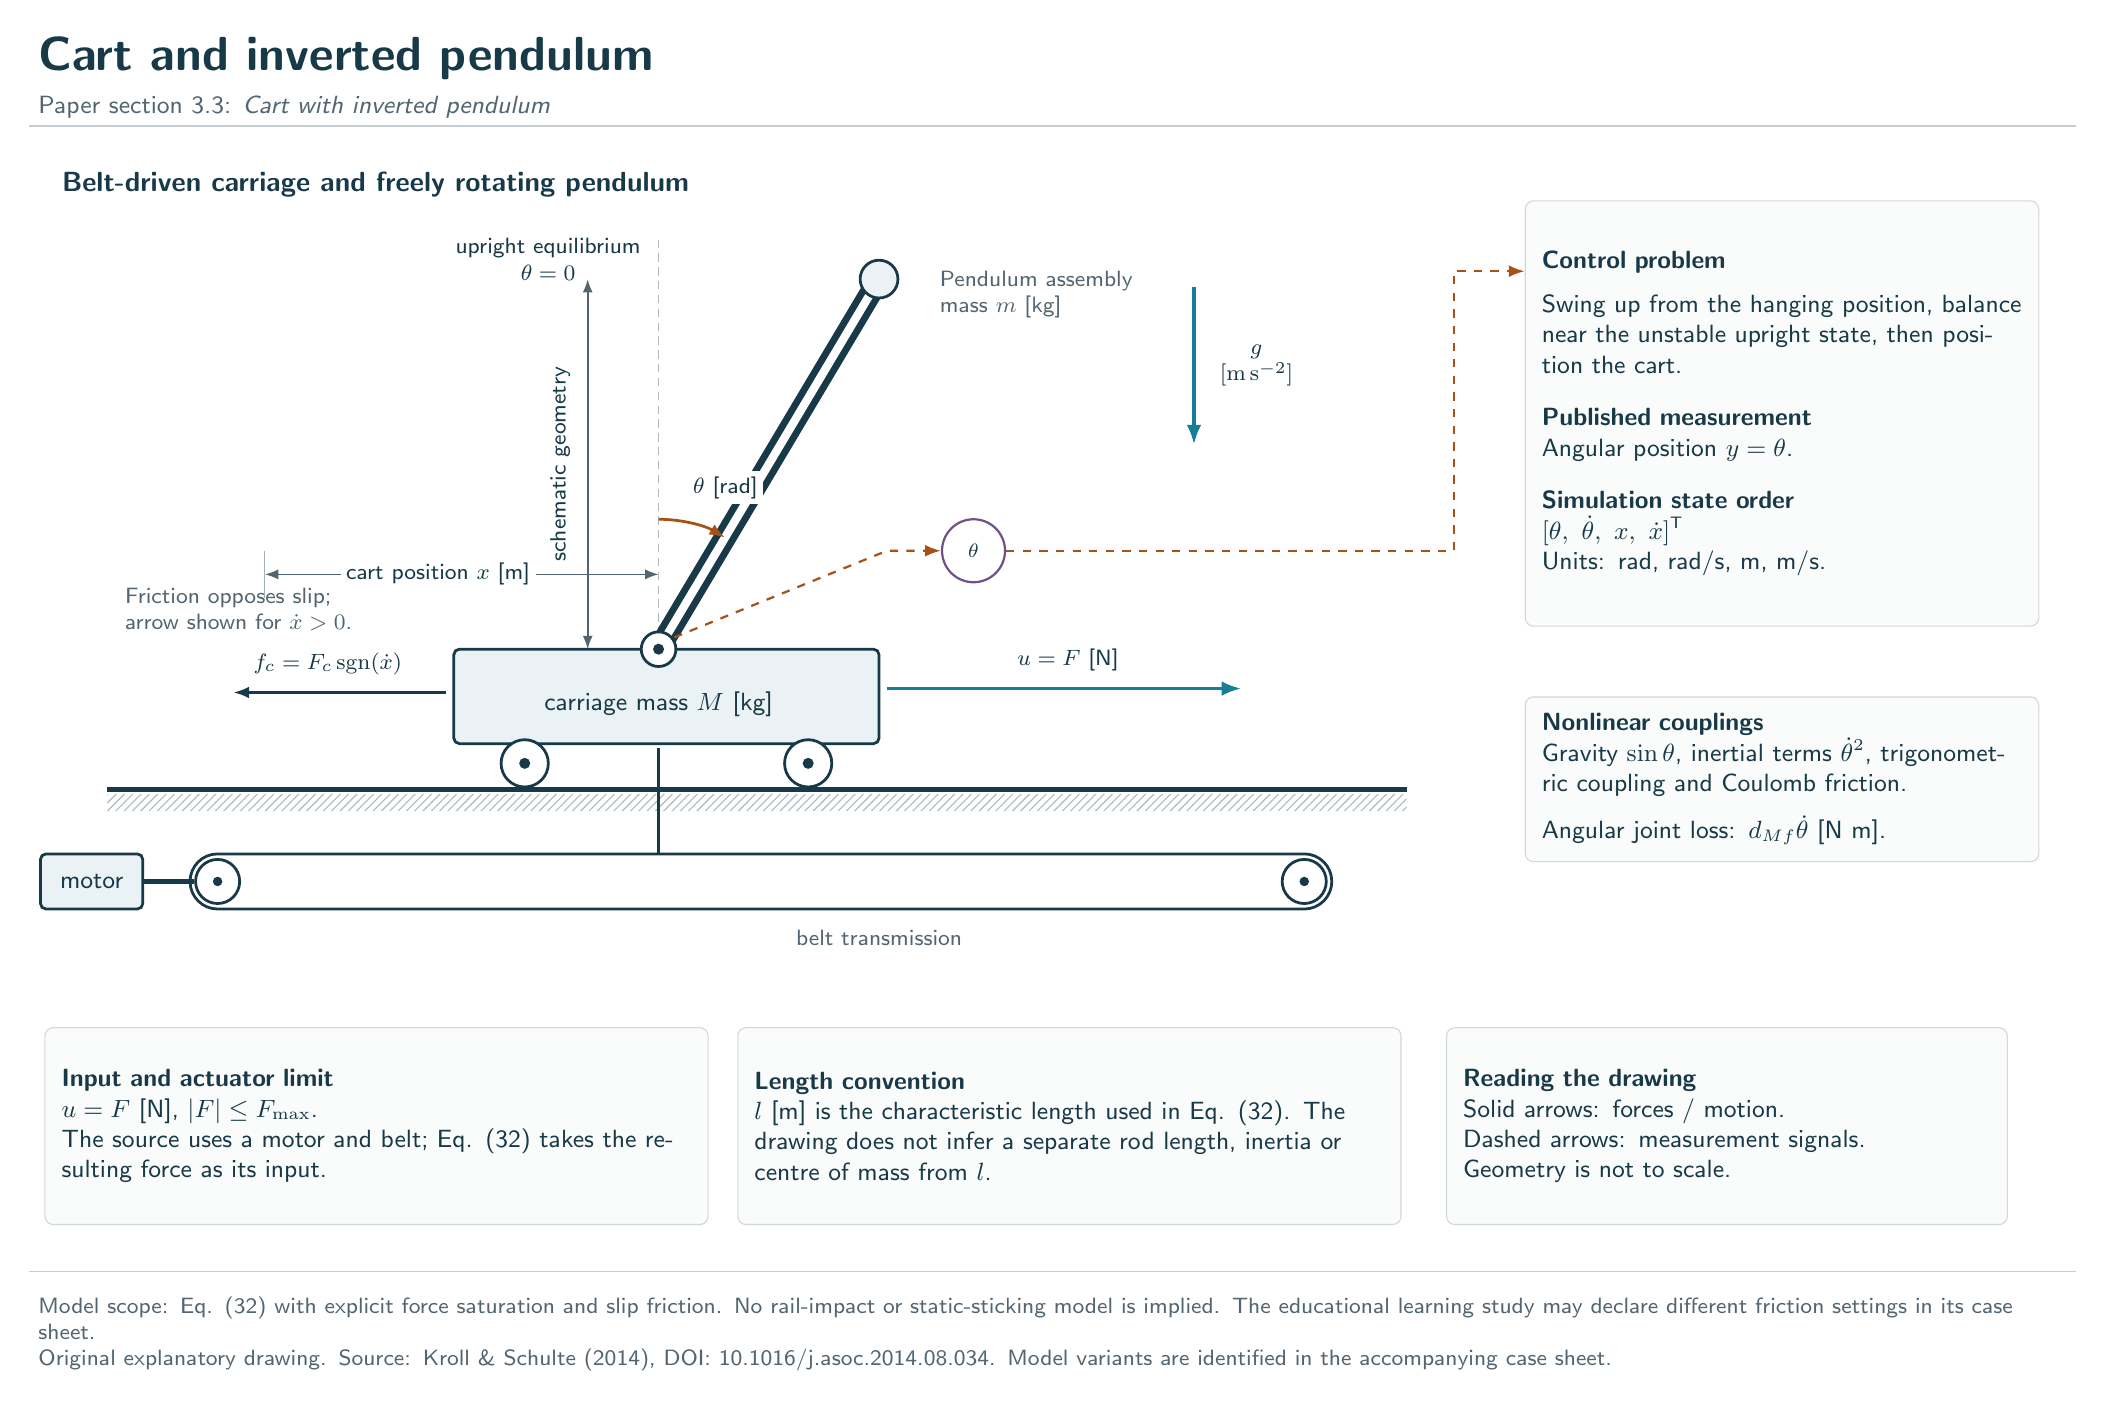
\begin{tikzpicture}[x=1cm,y=1cm]
\atlasheader{Cart and inverted pendulum}{3.3}{Cart with inverted pendulum}
% Coordinates are schematic; l is the characteristic length of Eq. (32).
\node[anchor=west,font=\sffamily\bfseries] at (.3,-2) {Belt-driven carriage and freely rotating pendulum};
\draw[ink!35,densely dashed] (8,-7.9)--(8,-2.7);
\node[labelbox,anchor=east] at (7.85,-2.95) {upright equilibrium\\$\theta=0$};
\draw[ink,line width=8pt] (8,-7.9)--(10.8,-3.2);
\draw[white,line width=3pt] (8,-7.9)--(10.8,-3.2);
\filldraw[fill=pale,draw=ink,line width=1pt] (10.8,-3.2) circle (.24);
\node[annotation,anchor=west,text width=3.4cm] at (11.45,-3.4) {Pendulum assembly\\mass $m$ [kg]};
\draw[dimension] (7.1,-7.9)--(7.1,-3.2);
\node[labelbox,rotate=90] at (6.75,-5.55) {schematic geometry};
\draw[control,-{Latex[length=2mm]},line width=1pt] (8,-6.25) arc[start angle=90,end angle=59.2,radius=1.65];
\node[labelbox] at (8.85,-5.85) {$\theta$ [rad]};
\draw[process] (14.8,-3.3)--(14.8,-5.3);
\node[labelbox,anchor=west] at (15.05,-4.3) {$g$\\$[\mathrm{m\,s^{-2}}]$};
% Carriage, pivot bearing and rail.
\filldraw[equipment] (5.4,-7.9) rectangle (10.8,-9.1);
\node at (8,-8.6) {carriage mass $M$ [kg]};
\filldraw[draw=ink,fill=white,line width=1pt] (8,-7.9) circle (.22);
\fill[ink] (8,-7.9) circle (.07);
\foreach \x in {6.3,9.9}{\filldraw[draw=ink,fill=white,line width=1pt] (\x,-9.35) circle (.3);\fill[ink] (\x,-9.35) circle (.07);}
\draw[ink,line width=1.8pt] (1,-9.68)--(17.5,-9.68);
\fill[pattern=north east lines,pattern color=ink!35] (1,-9.75) rectangle (17.5,-9.95);
\draw[process] (10.9,-8.4)--(15.4,-8.4);
\node[labelbox,anchor=south] at (13.2,-8.25) {$u=F$ [N]};
\draw[ink,-{Latex[length=2mm]},line width=1pt] (5.3,-8.45)--(2.6,-8.45);
\node[labelbox,anchor=south] at (3.8,-8.3) {$f_c=F_c\,\mathrm{sgn}(\dot x)$};
\node[annotation,anchor=west] at (1.1,-7.4) {Friction opposes slip;\\arrow shown for $\dot x>0$.};
\draw[dimension] (3,-6.95)--(8,-6.95);
\draw[ink!40] (3,-6.65)--(3,-7.25);
\node[labelbox] at (5.2,-6.95) {cart position $x$ [m]};
\draw[ink,line width=1pt] (2.4,-10.5)--(16.2,-10.5) arc[start angle=90,end angle=-90,radius=.35]--(2.4,-11.2) arc[start angle=270,end angle=90,radius=.35];
\foreach \x in {2.4,16.2}{\draw[ink,fill=white,line width=1pt] (\x,-10.85) circle (.28);\fill[ink] (\x,-10.85) circle (.06);}
\draw[ink,line width=1.3pt] (8,-9.15)--(8,-10.5);
\node[annotation,anchor=north] at (10.8,-11.35) {belt transmission};
\node[equipment,minimum width=1.3cm,minimum height=.7cm] at (.8,-10.85) {motor};
\draw[ink,line width=2pt] (1.45,-10.85)--(2.1,-10.85);
% Signal path is separate from the mechanical force arrow.
\node[instrument] (angle) at (12,-6.65) {$\theta$};
\draw[signal] (8.2,-7.75)--(10.9,-6.65)--(angle.west);
\draw[signal] (angle.east)--(18.1,-6.65)--(18.1,-3.1)--(19,-3.1);
\node[panel,anchor=north west,text width=6.1cm,minimum height=5.4cm,align=left] at (19,-2.2) {\textbf{Control problem}\\[5pt]
 Swing up from the hanging position, balance near the unstable upright state, then position the cart.\\[8pt]
 \textbf{Published measurement}\\Angular position $y=\theta$.\\[8pt]
 \textbf{Simulation state order}\\$[\theta,\ \dot\theta,\ x,\ \dot x]^{\mathsf T}$\\Units: rad, rad/s, m, m/s.};
\node[panel,anchor=north west,text width=6.1cm,align=left] at (19,-8.5) {\textbf{Nonlinear couplings}\\Gravity $\sin\theta$, inertial terms $\dot\theta^2$, trigonometric coupling and Coulomb friction.\\[6pt]Angular joint loss: $d_{Mf}\dot\theta$ [N m].};
\node[panel,anchor=north west,text width=8cm,minimum height=2.5cm,align=left] at (.2,-12.7) {\textbf{Input and actuator limit}\\$u=F$ [N], $|F|\leq F_{\max}$.\\The source uses a motor and belt; Eq. (32) takes the resulting force as its input.};
\node[panel,anchor=north west,text width=8cm,minimum height=2.5cm,align=left] at (9,-12.7) {\textbf{Length convention}\\$l$ [m] is the characteristic length used in Eq. (32). The drawing does not infer a separate rod length, inertia or centre of mass from $l$.};
\node[panel,anchor=north west,text width=6.7cm,minimum height=2.5cm,align=left] at (18,-12.7) {\textbf{Reading the drawing}\\Solid arrows: forces / motion.\\Dashed arrows: measurement signals.\\Geometry is not to scale.};
\atlasfooter{Model scope: Eq. (32) with explicit force saturation and slip friction. No rail-impact or static-sticking model is implied. The educational learning study may declare different friction settings in its case sheet.}
\end{tikzpicture}
\end{document}
